% !TEX root = ../main.tex
\chapter{Contexto y estado de la técnica}

Este capítulo presenta los fundamentos conceptuales y el estado actual de la técnica en computación cuántica aplicada a la ciencia de datos. Se revisan los trabajos previos más relevantes, se identifican las limitaciones de los enfoques existentes y se sitúa la contribución de este trabajo en el contexto académico y profesional actual.

\section{Antecedentes históricos}

El origen formal de la computación cuántica como disciplina se remonta a los trabajos de \cite{feynman1982}, quien propuso el uso de sistemas cuánticos para simular la naturaleza de forma eficiente, argumentando que un computador clásico no podía simular un sistema cuántico sin un coste exponencial. Poco después, \cite{deutsch1985} formalizó el concepto de computador cuántico universal y demostró la existencia de problemas que un computador cuántico podría resolver de forma más eficiente que cualquier computador clásico.

El interés por la computación cuántica se intensificó con los algoritmos de \cite{shor1994} y \cite{grover1996}, que demostraron aceleraciones exponenciales y cuadráticas respectivamente frente a los mejores algoritmos clásicos conocidos para factorización de enteros y búsqueda no estructurada. Estos resultados establecieron la viabilidad teórica de la ventaja cuántica y sentaron las bases para el desarrollo de hardware cuántico experimental. Los fundamentos formales del modelo de computación cuántica, incluyendo los postulados de la mecánica cuántica, las puertas cuánticas y los circuitos cuánticos, se encuentran desarrollados en detalle en \cite{nielsen2010}.

En paralelo, el campo del aprendizaje automático experimentó un crecimiento extraordinario impulsado por el aumento de la capacidad computacional y la disponibilidad de grandes volúmenes de datos \citep{jordan2015}. La confluencia de ambas disciplinas dio lugar al campo del aprendizaje automático cuántico (\textit{Quantum Machine Learning}, QML), cuyo objetivo es explorar si las capacidades de procesamiento cuántico pueden ofrecer ventajas en tareas de aprendizaje estadístico \citep{biamonte2017}.

\section{Computación cuántica en la era NISQ}

El estado actual del hardware cuántico se enmarca en lo que \cite{preskill2018} denominó la era NISQ (\textit{Noisy Intermediate-Scale Quantum}), caracterizada por dispositivos con entre 50 y varios cientos de qubits físicos, afectados por errores de decoherencia y ruido cuántico, y sin capacidad para implementar corrección de errores cuánticos a gran escala. Esta realidad impone restricciones fundamentales sobre la profundidad de los circuitos ejecutables y la fiabilidad de los resultados obtenidos.

\begin{figure}[!htbp]
\centering
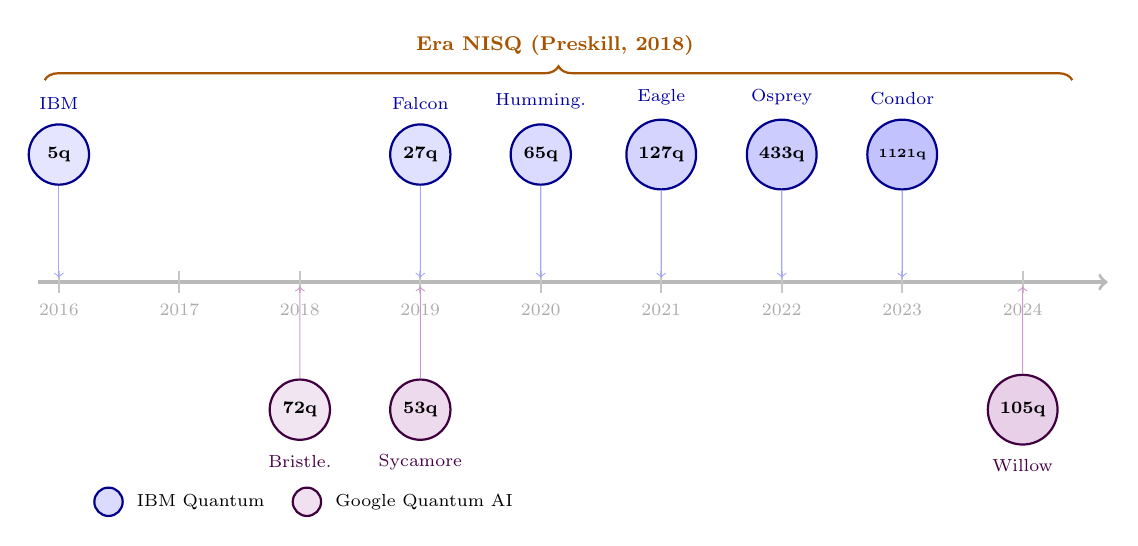
\begin{tikzpicture}[font=\scriptsize, thick, scale=0.9, transform shape]
  % Eje temporal
  \draw[->, very thick, gray!55] (-0.3, 0) -- (14.8, 0);

  % Marcas y etiquetas de año
  \foreach \yr/\x in {2016/0, 2017/1.7, 2018/3.4, 2019/5.1, 2020/6.8, 2021/8.5, 2022/10.2, 2023/11.9, 2024/13.6} {
    \draw[gray!45] (\x, -0.15) -- (\x, 0.15);
    \node[below=5pt, gray!65] at (\x, 0) {\yr};
  }

  % ── IBM (arriba) ──────────────────────────────────────────────────────────
  \node[circle, draw=blue!55!black, fill=blue!10, minimum size=0.85cm, align=center,
        font=\bfseries\scriptsize] (i1) at (0, 1.8) {5q};
  \node[above=2pt, blue!65!black, align=center, font=\scriptsize] at (i1.north) {IBM};
  \draw[->, blue!35, thin] (i1.south) -- (0, 0.06);

  \node[circle, draw=blue!55!black, fill=blue!12, minimum size=0.85cm, align=center,
        font=\bfseries\scriptsize] (i2) at (5.1, 1.8) {27q};
  \node[above=2pt, blue!65!black, align=center, font=\scriptsize] at (i2.north) {Falcon};
  \draw[->, blue!35, thin] (i2.south) -- (5.1, 0.06);

  \node[circle, draw=blue!55!black, fill=blue!14, minimum size=0.85cm, align=center,
        font=\bfseries\scriptsize] (i3) at (6.8, 1.8) {65q};
  \node[above=2pt, blue!65!black, align=center, font=\scriptsize] at (i3.north) {Humming.};
  \draw[->, blue!35, thin] (i3.south) -- (6.8, 0.06);

  \node[circle, draw=blue!55!black, fill=blue!17, minimum size=0.85cm, align=center,
        font=\bfseries\scriptsize] (i4) at (8.5, 1.8) {127q};
  \node[above=2pt, blue!65!black, align=center, font=\scriptsize] at (i4.north) {Eagle};
  \draw[->, blue!35, thin] (i4.south) -- (8.5, 0.06);

  \node[circle, draw=blue!55!black, fill=blue!20, minimum size=0.85cm, align=center,
        font=\bfseries\scriptsize] (i5) at (10.2, 1.8) {433q};
  \node[above=2pt, blue!65!black, align=center, font=\scriptsize] at (i5.north) {Osprey};
  \draw[->, blue!35, thin] (i5.south) -- (10.2, 0.06);

  \node[circle, draw=blue!55!black, fill=blue!24, minimum size=0.85cm, align=center,
        font=\bfseries\tiny] (i6) at (11.9, 1.8) {1121q};
  \node[above=2pt, blue!65!black, align=center, font=\scriptsize] at (i6.north) {Condor};
  \draw[->, blue!35, thin] (i6.south) -- (11.9, 0.06);

  % ── Google (abajo) ────────────────────────────────────────────────────────
  \node[circle, draw=violet!50!black, fill=violet!10, minimum size=0.85cm, align=center,
        font=\bfseries\scriptsize] (g1) at (3.4, -1.8) {72q};
  \node[below=2pt, violet!55!black, align=center, font=\scriptsize] at (g1.south) {Bristle.};
  \draw[->, violet!40, thin] (g1.north) -- (3.4, -0.06);

  \node[circle, draw=violet!50!black, fill=violet!14, minimum size=0.85cm, align=center,
        font=\bfseries\scriptsize] (g2) at (5.1, -1.8) {53q};
  \node[below=2pt, violet!55!black, align=center, font=\scriptsize] at (g2.south) {Sycamore};
  \draw[->, violet!40, thin] (g2.north) -- (5.1, -0.06);

  \node[circle, draw=violet!50!black, fill=violet!18, minimum size=0.85cm, align=center,
        font=\bfseries\scriptsize] (g3) at (13.6, -1.8) {105q};
  \node[below=2pt, violet!55!black, align=center, font=\scriptsize] at (g3.south) {Willow};
  \draw[->, violet!40, thin] (g3.north) -- (13.6, -0.06);


  % Llave "Era NISQ"
  \draw[decorate, decoration={brace, amplitude=5pt}, thick, orange!65!black]
    (-0.2, 2.85) -- (14.3, 2.85);
  \node[above=6pt, orange!65!black, font=\footnotesize\bfseries] at (7.0, 2.85)
    {Era NISQ (Preskill, 2018)};

  % Leyenda
  \node[circle, draw=blue!55!black, fill=blue!14, minimum size=0.4cm] at (0.7, -3.1) {};
  \node[right=2pt, font=\scriptsize] at (0.9, -3.1) {IBM Quantum};
  \node[circle, draw=violet!50!black, fill=violet!12, minimum size=0.4cm] at (3.5, -3.1) {};
  \node[right=2pt, font=\scriptsize] at (3.7, -3.1) {Google Quantum AI};
\end{tikzpicture}
\caption[Evolución del hardware cuántico en la era NISQ (2016--2024)]{Evolución del hardware cuántico en la era NISQ (2016--2024). Los nodos superiores (azul) corresponden a procesadores IBM Quantum; los inferiores (violeta) a Google Quantum AI. Se indica el año de presentación de cada procesador; los recuentos de qubits de IBM proceden de sus anuncios públicos. Los números indican el recuento de qubits físicos disponibles. \citet{arute2019} presentaron con Sycamore (2019) un experimento de muestreo de circuitos aleatorios que declararon fuera del alcance de la simulación clásica de entonces; \citet{pan2022} lo replicaron después con algoritmos clásicos mejorados. Willow (2024) se asocia al trabajo de \citet{willow2025} sobre corrección de errores por debajo del umbral del código de superficie.}
\label{fig:timeline_hardware}
\end{figure}

En respuesta a estas limitaciones, se han desarrollado los algoritmos variacionales cuánticos (\textit{Variational Quantum Algorithms}, VQA), que combinan un circuito cuántico parametrizado con un optimizador clásico en un bucle híbrido \citep{cerezo2021}. Entre los más destacados se encuentran el Quantum Approximate Optimization Algorithm (QAOA) \citep{farhi2014}, diseñado para problemas de optimización combinatoria, y el Variational Quantum Eigensolver (VQE) \citep{peruzzo2014}, orientado a la simulación de sistemas moleculares. Estos algoritmos son actualmente los candidatos más prometedores para demostrar ventaja cuántica práctica en hardware NISQ.

No obstante, la comunidad científica mantiene un debate activo sobre si los algoritmos NISQ pueden alcanzar ventaja cuántica genuina frente a los mejores algoritmos clásicos. \cite{mcclean2018} mostraron que, en circuitos parametrizados aleatorios, la probabilidad de que el gradiente sea distinto de cero con precisión fija es exponencialmente pequeña en el número de qubits (\textit{barren plateaus}), lo que dificulta el entrenamiento de los circuitos variacionales a medida que el número de qubits crece. \cite{cerezo2023} discuten además si los modelos libres de \textit{barren plateaus} pueden simularse eficientemente de forma clásica, lo que cuestiona qué ventaja pueden ofrecer.

\section{Aprendizaje automático cuántico}

El aprendizaje automático cuántico ha sido objeto de una revisión por parte de \cite{biamonte2017}, quienes identificaron cuatro categorías principales de algoritmos QML según la naturaleza del procesador (clásico o cuántico) y de los datos (clásicos o cuánticos). Para el contexto de este trabajo, el caso más relevante es el de datos clásicos procesados mediante algoritmos cuánticos (CQ en la nomenclatura de los autores: datos clásicos, procesador cuántico).

Los métodos basados en kernels cuánticos (\textit{Quantum Kernel Methods}) han recibido especial atención. \cite{schuld2021} propusieron interpretar los circuitos cuánticos como mapas de características (\textit{feature maps}) hacia espacios de Hilbert de alta dimensión, y \cite{havlicek2019} implementaron experimentalmente el estimador de kernel cuántico en un procesador superconductor, argumentando que ciertos mapas son difíciles de simular clásicamente. Sin embargo, \cite{huang2021} establecieron condiciones teóricas precisas bajo las cuales los kernels cuánticos pueden ofrecer una ventaja de aprendizaje sobre los kernels clásicos, concluyendo que dicha ventaja depende críticamente de la estructura geométrica de los datos de entrada.

En el contexto de la clasificación supervisada con datos reales, \cite{haug2023} propusieron el uso de medidas aleatorizadas para escalar los métodos de kernel cuántico a conjuntos de datos de gran tamaño, abordando uno de los principales cuellos de botella prácticos de estos métodos: el coste de estimar el kernel crece cuadráticamente con el tamaño del conjunto de datos. Su método reduce el tiempo de cómputo cuántico a escala lineal con dicho tamaño, aunque en general escala de forma exponencial con el número de qubits, y lo demostraron clasificando imágenes en un procesador cuántico de IBM.

\section{Optimización cuántica aplicada}

El QAOA, propuesto originalmente por \cite{farhi2014}, es un algoritmo híbrido cuántico-clásico que aproxima la solución de problemas de optimización combinatoria formulados como problemas de optimización cuadrática binaria sin restricciones (QUBO). Su aplicabilidad se extiende a problemas de relevancia empresarial como la optimización de rutas \citep{lucas2014}, la asignación de recursos, la segmentación de mercado y la optimización de carteras financieras.

\cite{zhou2020} estudiaron numéricamente el QAOA sobre MaxCut en grafos regulares, hasta $p\leq 50$ y $N\leq 22$ vértices, y propusieron estrategias heurísticas de inicialización de parámetros cuyo coste crece de forma polinómica en $p$; observaron además que la calidad de la solución mejora al aumentar la profundidad. No obstante, la ventaja cuántica del QAOA frente a los mejores algoritmos clásicos heurísticos sigue siendo una cuestión abierta para instancias de gran escala \citep{farhi2014}.

Desde una perspectiva aplicada, \cite{vikstaal2020} simularon el QAOA sobre instancias del problema de asignación de aeronaves a vuelos (\textit{tail-assignment}) derivadas de datos reales de una aerolínea, reducidas a 8, 15 y 25 qubits. Encontraron que repetidas ejecuciones identifican la solución factible con probabilidad cercana a uno, que los parámetros variacionales siguen patrones que permiten interpolarlos entre profundidades, y que la probabilidad de éxito por medición depende de la conectividad del grafo del problema. Estos resultados subrayan la importancia de realizar evaluaciones experimentales sobre datos reales más allá de las pruebas de concepto teóricas.

\section{Análisis crítico de los trabajos previos}

La revisión de la literatura permite identificar un conjunto de limitaciones recurrentes en los estudios existentes que este trabajo pretende abordar:

\begin{itemize}
    \item \textbf{Uso predominante de datos sintéticos o académicos}: la mayoría de los estudios comparativos utilizan conjuntos de datos de benchmarks estándar (Iris, MNIST, MaxCut), que no reflejan la complejidad y el ruido inherentes a los datos empresariales reales.

    \item \textbf{Ausencia de comparación sistemática con métodos clásicos consolidados}: muchos trabajos evalúan el rendimiento cuántico de forma aislada, sin contrastar con técnicas clásicas de referencia como SVM, Random Forests o algoritmos genéticos en las mismas condiciones experimentales.

    \item \textbf{Foco en la viabilidad teórica más que en la aplicabilidad práctica}: los análisis de ventaja cuántica suelen estar formulados en términos asintóticos o bajo supuestos ideales de hardware, sin considerar las restricciones reales de los dispositivos NISQ actuales \citep{preskill2018}.

    \item \textbf{Escasa consideración de la integración en pipelines productivos}: los trabajos existentes raramente abordan la cuestión de cómo los módulos cuánticos podrían integrarse en arquitecturas de análisis de datos clásicas ya existentes en entornos empresariales.
\end{itemize}

Este trabajo contribuye a superar estas limitaciones mediante un diseño experimental que combina datos reales de negocio, comparación directa con métodos clásicos de referencia y una evaluación orientada a la viabilidad de integración práctica.